
In this section, we will give you an overview of Clang's structures and organizations. We will briefly introduce some of the important components or subsystems, before using dedicated sections or chapters to expand them further in later parts of this book. We hope this will give you some idea of Clang's internals and how they will benefit your development.

First, let's look at the big picture. The following diagram shows the high-level structure of Clang:

\hspace*{\fill} \\ %插入空行
\begin{center}
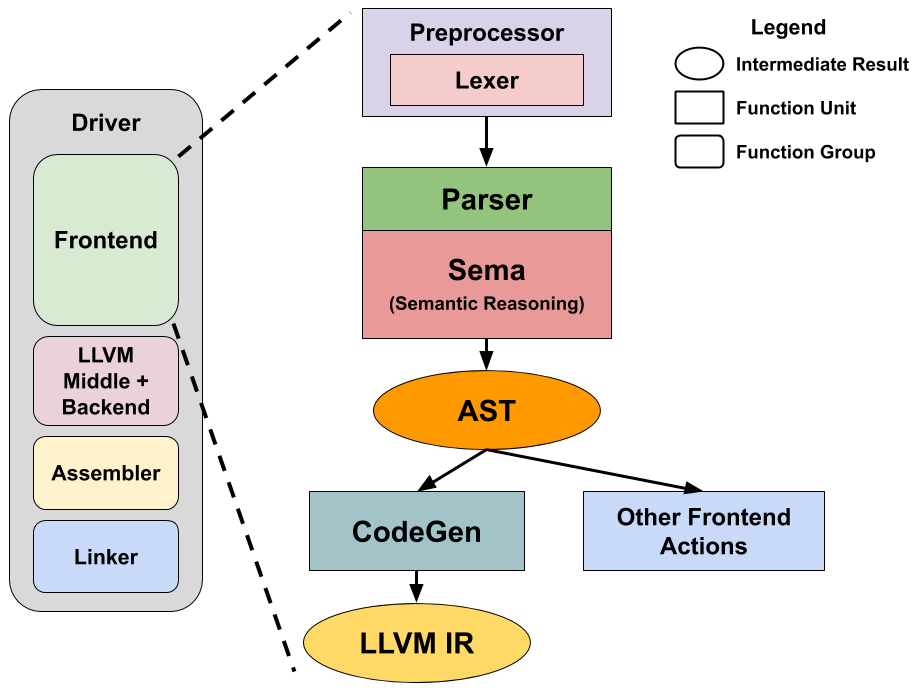
\includegraphics[width=0.9\textwidth]{content/2/chapter5/images/1.png}\\
Figure 5.1 – High-level structure of Clang
\end{center}

As explained in the legend, rectangles with rounded corners represent subsystems that might consist of multiple components with similar functionalities. For example, the frontend can be further dissected into components such as the preprocessor, parser, and code generation logic, to name a few. In addition, there are intermediate results, depicted as ovals in the preceding diagram. We are especially interested in two of them – Clang AST and LLVM IR. The former will be discussed in depth in Chapter 7, Handling AST, while the latter is the main character of Part 3, Middle-End Development, which will talk about optimizations and analyses you can apply to LLVM IR.

Let's start by looking at an overview of the driver. The following subsections will give you a brief introduction to each of these driver components.


\subsubsubsection{5.2.1\hspace{0.2cm}Driver}

A common misunderstanding is that clang, the executable, is the compiler frontend. While clang does use Clang's frontend components, the executable itself is actually a kind of program called a compiler driver, or driver for short.

Compiling source code is a complex process. First, it consists of multiple phases, including the following:

\begin{itemize}
\item Frontend: Parsing and semantic checking
\item Middle-end: Program analysis and optimization
\item Backend: Native code generation
\item Assembling: Running the assembler
\item Linking: Running the linker
\end{itemize}

Among these phases and their enclosing components, there are countless options/arguments and flags, such as the option to tell compilers where to search for include files (that is, the -I command-line option in GCC and Clang). Furthermore, we hope that the compiler can figure out the values for some of these options. For example, it would be great if the compiler could include some folders of C/C++ standard libraries (for example, /include and /usr/include in Linux systems) in the header file search paths by default, so that we don't need to assign each of those folders manually in the command line. Continuing with this example, it's clear that we want our compilers to be portable across different operating systems and platforms, but many operating systems use a different C/C++ standard library path. So, how do compilers pick the correct one accordingly?

In this situation, a driver is designed to come to the rescue. It's a piece of software that acts as a housekeeper for core compiler components, serving them essential information (for example, a OS-specific system include path, as we mentioned earlier) and arranging their executions so that users only need to supply important command-line arguments. A good way to observe the hard work of a driver is to use the -\#\#\# command-line flag on a normal clang invocation. For example, you could try to compile a simple hello world program with that flag:

\begin{tcblisting}{commandshell={}}
$ clang++ -### -std=c++11 -Wall ./hello_world.cpp -o hello_world
\end{tcblisting}

The following is part of the output after running the preceding command on a macOS computer:

\begin{tcblisting}{commandshell={}}
"/path/to/clang" "-cc1" "-triple" "x86_64-apple-macosx11.0.0"
"-Wdeprecated-objc-isa-usage" "-Werror=deprecated-objcisa-usage" 
"-Werror=implicit-function-declaration" "-emitobj" "-mrelax-all" 
"-disable-free" "-disable-llvm-verifier" … "-fno-strict-return" 
"-masm-verbose" "-munwind-tables" "-target-sdk-version=11.0" … "-resource-dir"
"/Library/Developer/CommandLineTools/usr/lib/clang/12.0.0" "-isysroot"
"/Library/Developer/CommandLineTools/SDKs/MacOSX.sdk" "-I/usr/local/include" 
"-stdlib=libc++" … "-Wall" "-Wno-reorderinit-list" "-Wno-implicit-int-float-
conversion" "-Wno-c99-designator" … "-std=c++11" "-fdeprecated-macro" 
"-fdebugcompilation-dir" "/Users/Rem" "-ferror-limit" "19" "-fmessage-length" 
"87" "-stack-protector" "1" "-fstackcheck" "-mdarwin-stkchk-strong-link" … 
"-fexceptions" … "-fdiagnostics-show-option" "-fcolor-diagnostics" "-o" 
"/path/to/temp/hello_world-dEadBeEf.o" "-x" "c++" "hello_world.cpp"…
\end{tcblisting}

These are essentially the flags being passed to the real Clang frontend after the driver's translation. While you don't need to understand all these flags, it's true that even for a simple program, the compilation flow consists of an enormous amount of compiler options and many subcomponents.

The source code for the driver can be found under clang/lib/Driver. In Chapter 8, Working with Compiler Flags and Toolchains, we will look at this in more detail.

\subsubsubsection{5.2.2\hspace{0.2cm}Frontend}

A typical compiler textbook might tell you that a compiler frontend consists of a lexer and a parser, which generates an abstract syntax tree (AST). Clang's frontend also uses this skeleton, but with some major differences. First, the lexer is usually coupled with the preprocessor, and the semantic analysis that's performed on the source code is detached into a separate subsystem, called the Sema. This builds an AST and does all kinds of semantic checking.

\hspace*{\fill} \\ %插入空行
\noindent
\textbf{Lexer and preprocessor}

Due to the complexity of programming language standards and the scale of real-world source code, preprocessing becomes non-trivial. For example, resolving included files becomes tricky when you have 10+ layers of a header file hierarchy, which is common in large-scale projects. Advanced directives such as \#pragma can be challenged in cases where OpenMP uses \#pragma to parallelize for loops. Solving these challenges requires close cooperation between the preprocessor and the lexer, which provides primitives for all the preprocessing actions. Their source code can be found under clang/lib/Lex. In Chapter 6, Extending the Preprocessor, you will become familiar with preprocessor and lexer development, and learn how to implement custom logic with a powerful extension system.

\hspace*{\fill} \\ %插入空行
\noindent
\textbf{Parser and Sema}

Clang's parser consumes token streams from the preprocessor and lexer and tries to realize their semantic structures. Here, the Sema sub-system performs more semantic checking and analysis from the parser's result before generating the AST. Historically, there was another layer of abstraction where you could create your own parser action callbacks to specify what actions you wanted to perform when certain language directives (for example, identifiers such as variable names) were parsed.

Back then, Sema was one of these parser actions. However, later on, people found that this additional layer of abstraction was not necessary, so the parser only interacts with Sema nowadays. Nevertheless, Sema still retains this kind of callback-style design. For example, the clang::Sema::ActOnForStmt(…) function (defined in clang/lib/Sema/SemaStmt.cpp) will be invoked when a for loop structure is parsed. It will then do all kinds of checking to make sure the syntax is correct and generate the AST node for the for loop; that is, a ForStmt object.

\hspace*{\fill} \\ %插入空行
\noindent
\textbf{AST}

The AST is the most important primitive when it comes to extending Clang with your custom logic. All the common Clang extensions/plugins that we will introduce operate on an AST. To get a taste of AST, you can use the following command to print out the an AST from the source code:

\begin{tcblisting}{commandshell={}}
$ clang -Xclang -ast-dump -fsyntax-only foo.c
\end{tcblisting}

For example, on my computer, I have used the following simple code, which only contains one function:

\begin{lstlisting}[style=styleCXX]
int foo(int c) { return c + 1; }
\end{lstlisting}

This will yield the following output:

\begin{tcblisting}{commandshell={}}
TranslationUnitDecl 0x560f3929f5a8 <<invalid sloc>> <invalid
sloc>
|…
`-FunctionDecl 0x560f392e1350 <./test.c:2:1, col:30> col:5 foo
'int (int)'
  |-ParmVarDecl 0x560f392e1280 <col:9, col:13> col:13 used c
'int'
  `-CompoundStmt 0x560f392e14c8 <col:16, col:30>
    `-ReturnStmt 0x560f392e14b8 <col:17, col:28>
      `-BinaryOperator 0x560f392e1498 <col:24, col:28> 'int' '+'
        |-ImplicitCastExpr 0x560f392e1480 <col:24> 'int' <LValueToRValue>
        |   `-DeclRefExpr 0x560f392e1440 <col:24> 'int' lvalue ParmVar 0x560f
              392e1280 'c' 'int'
        `-IntegerLiteral 0x560f392e1460 <col:28> 'int' 1
\end{tcblisting}

This command is pretty useful because it tells you the C++ AST class that represents certain language directives, which is crucial for writing AST callbacks – the core of many Clang plugins. For example, from the previous lines, we can know that a variable reference site (c in the c + 1 expression) is represented by the DeclRefExpr class.

Similar to how the parser was organized, you can register different kinds of ASTConsumer instances to visit or manipulate the AST. CodeGen, which we will introduce shortly, is one of them. In Chapter 7, Handling AST, we will show you how to implement custom AST processing logic using plugins.

\hspace*{\fill} \\ %插入空行
\noindent
\textbf{CodeGen}

Though there are no prescriptions for how you should process the AST (for example, if you use the -ast-dump command-line option shown previously, the frontend will print the textual AST representation), the most common task that's performed by the CodeGen subsystem is emitting the LLVM IR code, which will later be compiled into native assembly or object code by LLVM.

\subsubsubsection{5.2.3\hspace{0.2cm}LLVM,组译器和连接器}

Once the LLVM IR code has been emitted by the CodeGen subsystem, it will be processed by the LLVM compilation pipeline to generate native code, either assembly code or object code. LLVM provides a framework called the MC layer, in which architectures can choose to implement assemblers that have been directly integrated into LLVM's pipeline. Major architectures such as x86 and ARM use this approach. If you don't do this, any textual assembly code that's emitted at the end of LLVM's pipeline needs to be processed by external assembler programs invoked by the driver

Despite the fact that LLVM already has its own linker, known as the LLD project, an integrated linker is still not a mature option yet. Therefore, external linker programs are always invoked by the driver to link the object files and generate the final binary artifacts.

\begin{tcolorbox}[colback=blue!5!white,colframe=blue!75!black, fonttitle=\bfseries,title=External versus integrated]
\hspace*{0.7cm}Using external assemblers or linkers means invoking a separate process to run the program. For example, to run an external assembler, the frontend needs to put assembly code into a temporary file before launching the assembler with that file path as one of its command-line arguments. On the other hand, using integrated assemblers/linkers means the functionalities of assembling or linking are packaged into libraries rather than an executable. So, at the end of the compilation pipeline, LLVM will call APIs to process the assembly code's in-memory instances to emit object code. The advantage of this integrated approach is, of course, saving many indirections (writing into temporary files and reading them back right away). It also makes the code more concise to some extent.
\end{tcolorbox}

With that, you have been given an overview of a normal compilation flow, from the source code all the way to the native code. In the next section, we will go beyond the clang executable and provide an overview of the tooling and extension options provided by Clang. This not only augments the functionalities of clang, but also provides a way to use Clang's amazing techniques in out-of-tree projects.





























